%\section{Indicadores Estatísticos Descritivos}
%
%Falar nesta secçaõ sobre:
%
%\begin{itemize}
%	\item Boxplot / diagrama de extremos e quartis
%	\item qunatis e as várias definições
%	\item outliers
%	\item função inversa generalizada
%	\item missing values
%	\item medidas de risco
%\end{itemize}
%
%
%\begin{figure}[H]
%	\centering
%	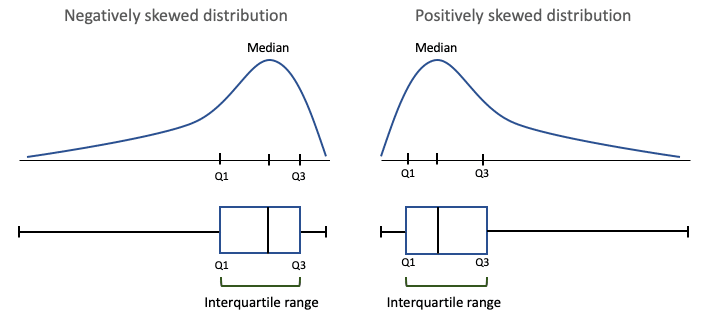
\includegraphics[width=0.7\textwidth]{imagens/skewed.png}
%	\caption{}
%	\label{}
%\end{figure}
%
%FAZER REPRESENTACAO GRÁFICA DESTE TIPO PARA JUSTIFICAR O PARÁGRAFO QUE ANTECEDE O PLOT DA COMPARACAO DA MEDIA, MEDIANA E DP DO NEC POR CPV DA FLAG R019

Um boxplot, também conhecido como diagrama de extremos e quartis, é uma ferramenta gráfica usada em Estatística para visualizar a distribuição de um conjunto de dados \cite{casella2002statistical} \cite{ross2014introduction}. A informação fornecida pelo boxplot é feita através dos seus componentes: 

\begin{my_itemize}
	
	\item Quartis: Os quartis são os valores que dividem um conjunto de dados ordenados em quatro partes iguais, cada uma contendo 25\% dos dados. Para calculá-los, é necessário organizar os dados por ordem crescente.O primeiro quartil (Q1), também conhecido como quartil inferior, é o valor abaixo do qual se encontram 25\% dos dados ordenados. O segundo quartil (Q2), ou mediana, é o valor abaixo do qual se encontra 50\% dos dados ordenados. O terceiro quartil (Q3), conhecido como quartil superior, é o valor abaixo do qual se encontra 75\% dos dados ordenados.
	
	\item Caixa: Representa o intervalo interquartil (IQR). Neste intervalo estão contidos  todos os dados cujo valor é superior ao primeiro quartil (Q1) e inferior ao terceito quartil (Q3), contemplando 50\% dos dados. A caixa permite verificar a dispersão dos dados: uma caixa maior indica uma maior variabilidade dos dados, enquanto que uma caixa menor indica uma menor variabilidade dos dados. 
	
	\item Mediana: É a linha que se encontra dentro da caixa e é apelidade de mediana (Q2). Esta linha divide o conjunto de dados em duas metadas iguais. É a partir da localização da mediana dentro da caixa que se pode observar a presença, ou não, de assimetria na distribuição dos dados. Se a linha se encontrar no meio, ou muito perto do meio, da caixa significa que a distribuição dos dados é simétrica. Por outro lado, se esta estiver deslocada para um dos lados significa que o conjunto de dados é assimétrico. 
	
	\item Extremidades (Whiskers): São as linhas que se estendem desde os primeiro e terceiro quartil até os valores mais extremos do conjunto de dados que não sejam considerados outliers. Existem diferentes formas de definir estas extremidadas\cite{spe},  mas, geralmente, são definidos como: $[Q1 - 1.5IQR, Q3 + IQR]$. As extremidades também permitem verificar a variabilidade dos dados. 
	
	\item Outliers: São todos os pontos que não são abrangidos pelas extremidades. São valores bastante diferentes dos demais e são representados por pontos individuais. A existência de um elevado número de outliers pode indicar a presença de distribuições com caudas longas e a presença de valores extremos.
	
\end{my_itemize}


Os boxplots permitem ter uma visão da distribuição dos dados, identificando rapidamente outliers e assimetrias para uma amostra com um número de observações estatisticamente significativo. Contudo, não detalha a distribuição de uma forma completa e, por isso, é frequentemete acompanhado de um histograma.



\begin{figure}[H]
	\centering
	\includegraphics[width=\textwidth]{imagens/stats/hist2.png}
	\caption{Exemplo de ilustração de histograma e boxplot para diferentes distribuições.}
	\label{fig:histos}
\end{figure}


Na Figura \ref{fig:histos} podem ser observadas três cenários distintos. Cada uma das amostras é composta por 1000 pontos gerados a partir das bibliotecas Numpy e Scipy do Python \cite{python}. A primeira amostra foi gerada a partir de uma distribuição normal com valor médio 0 e uma variância de 0.5, a segunda a partir de uma distribuição normal com valor médio 0 e variância 1 e a terceira a partir de uma distribuição normal assimétrica, usando o módulo scipy.stats.skewnorm. A partir da observação dos dois primeiros gráficos, verifica-se que a distância interquartil do primeiro é inferior à do segundo, resultado de uma menor variância/ maior concentração dos dados. No terceiro gráfico encontra-se uma distribuição assimétrica à esquerda. Através do seu boxplot, verifica-se que os whsikers não têm o mesmo tamanho e a mediana encontra-se mais próxima do primeiro quartil do que do terceiro. 


\section{Outliers}

























